\documentclass{article}

\usepackage{bookman}

% acentuação
\usepackage[utf8]{inputenc}
\usepackage{indentfirst}
\usepackage{xspace}
%\usepackage{chicago}
\usepackage{url}
\usepackage{setspace}
\usepackage{graphicx}

\usepackage{fancybox}
\usepackage{amsmath}
\usepackage{amsfonts}
\usepackage[bbgreekl]{mathbbol}
\usepackage{amssymb}
\usepackage{url}
\usepackage{multirow}
\usepackage{booktabs}
\usepackage{paralist}

\usepackage{color}
\usepackage{subfigure}
\definecolor{red}{rgb}{0.9,0.1,0.1}
\definecolor{blue}{rgb}{0,0.1,0.8}

%%% cria links no arquivo .pdf
%%% comentar as linhas na versão para impressao
\usepackage[pdftex, plainpages=false, hyperfootnotes=false]{hyperref}
\hypersetup{colorlinks=true, linkcolor=blue, citecolor=blue, urlcolor=blue}

%%% bibliografia
%\usepackage{natbib}
\usepackage[sf,outermarks,clearempty]{titlesec}

\usepackage[pdftex]{geometry}
  \geometry{a4paper,left=3cm,right=2cm,top=3cm,bottom=3cm,twoside}

\usepackage{acronym}


\usepackage{eqparbox,array}

\usepackage{comment}
\usepackage{fontenc}
\usepackage{inputenc}
\usepackage{listing}
\usepackage{listings}
\usepackage{framed}


\acrodef{CBIR}{Content-based image retrieval}
\acrodef{MAM}{Metric Access Method}
\acrodef{AM}{Access Method}
\acrodef{SAM}{Spatial Access Method}
\acrodef{MST} {Minimum Spanning Tree}
\acrodef{IR} {Information Retrieval}
\acrodef{NDC} {Number of Distance Calculations}
\acrodef{LAESA} {Linear Approximating Eliminating Search Algorithm}
\acrodef{AESA} {Approximating Eliminating Search Algorithm}
\acrodef{RNG} {Relative Neighborhood Graph}
\acrodef{DT} {Delaunay Triangulation}
\acrodef{GG} {Gabriel Graph}
\acrodef{UG} {Urquhart Graph}
\acrodef{SAT} {Spacial Approximation Tree}
\acrodef{RNDF} {Relative Neighborhood Density Factor}
\acrodef{NN} {Nearest Neighbor}
\acrodef{NAG} {Neighborhood Approximation Graph}
\acrodef{HRG} {Hyperspherical Region Graph}
\acrodef{NA-Graph} {Neighborhood Approximation Graph}
\acrodef{DA} {Disk Access}
\acrodef{DTW} {Dynamic Time Warping}
\acrodef{LSH} {Locality Sensitive Hashing}
\acrodef{CNN} {Convolutional Neural Network}
\acrodef{CNNs} {Convolutional Neural Networks}

%\newcommand{ \Correction }[ 1 ] {\textcolor{black}{#1}}
%\newcommand{ \NewMaterial }[ 1 ] {\textcolor{black}{#1}}
%\newcommand{ \ConnectDots }[ 1 ] {\textcolor{black}{#1}}
%\newcommand{ \NewMaterialGPU }[ 1 ] {\textcolor{black}{#1}}
%\newcommand{ \Error }[ 1 ] {\textcolor{black}{#1}}


\acrodef{CBIR} {Content-based Image Retrieval}
\acrodef{MAM}  {Métodos de Acceso Métrico}
\acrodef{SAM}  {Métodos de Acceso Espacial}
\acrodef{MAE}  {Métodos de Acesso Espaciais}

\acrodef{DTW}  {Dynamic Time Warping}
\acrodef{LSH}  {Locality Sensitive Hashing}
\newenvironment{Figure}
  {\par\medskip\noindent\minipage{\linewidth}}
  {\endminipage\par\medskip}

\usepackage{courier}
\definecolor{darkgreen}{rgb}{0,0.6,0.1}
\definecolor{gray}{rgb}{0.75,0.75,0.75}


\title{A Small \LaTeX{} Article Template\thanks{To your mother}}
\author{Your Name  \\
	Your Company / University  \\
	\and
	The Other Dude \\
	His Company / University \\
	}

\date{\today}
% Hint: \title{what ever}, \author{who care} and \date{when ever} could stand
% before or after the \begin{document} command
% BUT the \maketitle command MUST come AFTER the \begin{document} command!
\begin{document}

\maketitle


\begin{abstract}
Short introduction to subject of the paper \ldots
\end{abstract}





\section{Introduction}\label{sec:intro}

The increasing availability of data in diverse domains has created a necessity to develop techniques and methods to discover knowledge from massive volumes of complex data, motivating many research works in databases, machine learning, and information retrieval communities.  This has driven the development of scalable and efficient techniques to organize and retrieve this kind of data. Similarity search has been the traditional approach for information retrieval.  Although several similarity search algorithms have been proposed to speed up similarity queries, most of them are either affected by the well-known ``curse of dimensionality''.  Retrieve  complex data causes   stability problems  when the data dimensionality is very high \cite{aleman_high_dimensional}.  %Some studies have shown that the idea of data representation with hyper spherical or rectangular region hierarchies can deteriorate similarity queries even compared with sequential search \cite{aleman_high_dimensional}.

%Considering that similarity is the instinctive criterion by which people make comparisons, the information retrieval communities use similarity to organize and search for data.    However, even though similarity is an intuitive measure for comparisons, it causes some difficulties on representing complex data and with the stability of the algorithms when the data dimensionality is very high (the ``curse of dimensionality'').  Although many research works have been conducted on developing efficient index structures and similarity search algorithms, only a few of them present theoretical guaranty of asymptotic stability for high-dimensional data.

%% WHAT'S WRONG WITH TREES & CURSE OF HIGH DIMENSIONALITY DATA (mine)
%Many solutions response similarity queries taking advantage of index structures. Trees are the most common index structures for these domains. These solutions based on hierarchies can be overcome by sequential search. The main reason is that, in high dimensional data, most of the time spent during the search process is the filtering step in which it ensures that the current result is the correct answer \cite{WhatsWrong}. Not all applications require accurate answers. Hence,  most of the time approximate solutions are  preferable to reduce the effects of the ``curse of dimensionality''. These approximate solutions are applied in large-scale problems where speed is more important than accuracy. In this context, we need to needs to optimize the balance between time and query result quality.

One of the few approaches that ensure an approximate solution with sublinear search cost for high-dimensional data is the Locality Sensitive Hashing (LSH) \cite{hashing_algoritghms_survey}. LSH is based on the idea that closeness between two objects is usually preserved by a random projection operation. In other words, if two objects are close together in their original space, then these two objects will remain close after a scalar projection operation. However, it presents some difficulties for approximate kNN queries, in particular, related to data domain parameter dependence and quality results. Therefore, in complex domains, in particular, in high dimensional data problems, an approximate solution with a solid theoretical analysis may be the best option in many application areas because of their efficiency in time and space.


 %% LSH
% Different approaches have been studied to solve the ``curse of dimensionality''. One of the research lines is to try to avoid the dimensionality problem by relaxing the query precision to speed up the query time. Potentially, this approach is feasible for applications that do not require exact answers and for which speed is more important than search accuracy. Moreover, the metric space definition already leads to an approximation of the true answer, and thus a second approximation at search time may be acceptable \cite{cit:avez99searching}.



 %In this direction, \acf{LSH} \cite{lsh} is one of the recent hash-based techniques proposed to organize and query high-dimensional data. Indeed, LSH is one of the few techniques that provide solid theoretical analysis and predictable loss of accuracy in the results. To answer similarity queries, \ac{LSH} searches only regions, which are represented by buckets, to which the query object is hashed (i.e., the candidate buckets containing the dataset objects with a high probability of similarity to the query object). Therefore, there is no need to fully explore the index data, and only the objects into the candidate buckets require further processing.

%% CNN %%

On the other hand, in Machine Learning traditionally images are often described by the hand-craft visual features.  However, these hand-craft features cannot well reveal the high-level semantic meaning (labels or tags) of images, and often limit the performance of image retrieval \cite{Li:2015:RSS:2881665.2882186}.   Inspired by recent advances in \acf{CNN}  \cite{ImageNet}, many methods solved the problem of precision of similarity retrieval by using CNN  as feature extractor and then  build a compact similarity-preserving hash code for fast image retrieval.   Again, hashing is widely used for large-scale image retrieval as well as video and document searches because the compact representation of hash code is essential for data storage and reasonable for query searches \cite{conf/cvpr/ShenSLS15}.  However, some drawbacks based  on these supervised hashing methods have not been solved entirely, as follows:
 

\begin{itemize}


 
\item[-]  There is a trade-off between classification error and quantization error: activations of lower layers are more general-purpose \cite{DBLP:journals/corr/YosinskiCBL14}, so training is more effective. However lower layers have larger  activations maps (many nodes), which are harder to encode which leads to a compromise.

 
\item[-]  There is a dependency on parameter values  for approximate similarity search schemes based on LSH, which determine the number of hash functions and number of hash tables.

\end{itemize}


 
 This paper proposes a novel supervised hashing technique,  named  Deep frActal based  Hashing (DAsH),  designed to perform scalable approximate similarity search. The contributions of our work are as follows. First,  we introduce and define a  scheme based on CNN and optimized using fractal theory. To overcome the limitation of large activations on lower layers of CNN (output of the last convolutional layer) we reduce its dimensionality using autoencoders  to the optimal sub-space. Then we index this new representation with LSH scheme.  Second, we present a novel method, based on fractal theory, which allow us to can find the optimal number of hash functions for an approximate similarity search scheme based on LSH.

 
The paper is organized as follows. Section 2 summarizes the background for this work. Section 3 describes the proposed technique and Section 4 reports experimental results on real and synthetic datasets. Finally, we conclude in Section 5.
 

 
\section{Locality Sensitive Hashing}\label{sec:background}

Previous work \cite{hashing_algoritghms_survey} has explored the idea of hashing objects and grouping them into buckets with the goal of performing approximate similarity search within buckets associated with the query element.  The idea behind LSH is that if two objects are close together in their original space, then these two objects will remain close after a scalar projection operation. Hence, let $h(x)$ be a hash function that maps a d-dimensional point $x$ to a one-dimensional value. The function $h(x)$ is said to be \textit{locality sensitive} if the probability of mapping two d-dimensional points $x_1$, $x_2$ to the same value grows as their distance $d(x_1, x_2)$ decreases. 

LSH based methods report efficient results when adequate values for $m$ (number of hash functions) and $L$ (number of indexes) are chosen. The $E^2$-LSH algorithm find the best value for  $m$ and $L$ by experimentally evaluating the cost of calculation for samples in the given dataset.  Basically, the tuning parameter of LSH is chosen as a function of the dataset to minimize the running time  of a query  while the space requirement is within the memory bounds \cite{LSHBook}.  


\subsection{Fractal Theory}
 

A fractal is characterized by the self-similarity property, i.e., it is an object that presents roughly the same characteristics when analyzed over a broad range of scales \cite{DBLP:journals/jidm/TrainaTWF10}. From the Fractal Theory, the Correlation Fractal Dimension $\mathfrak{D}$ is particularly useful for data analysis, since it can be applied to estimate the intrinsic dimension of real datasets that exhibit fractal behavior, i.e., exactly or statistically self-similar datasets \cite{DBLP:fractal2016}.   It has been shown that, given a set of $N$ objects in a dataset with a distance function $d(x,y)$, the average number of $k$ neighbors within a given distance $r$ is proportional to $r$ raised to $\mathfrak{D}$. Thus, the pair-count $PC(r)$ of pairs of elements within distance $r$ follows the power law:
\begin{equation}\label{eq:fractal}
       PC(r) = K_p \times r^{\mathfrak{D}}
    \end{equation}

     where, $K_p$ is a proportionality constant, and $\mathfrak{D}$ is the correlation fractal dimension of the dataset.
    Consequently, a fractal is defined by the self-similarity property, that is the main characteristic that represents exactly or statistically  the similarity between the parts to the whole fractal.

 
\subsection{Using Fractals to estimate LSH parameters}

%The idea to use Correlation Fractal Dimension to compute the LSH parameters take advantage of fractal theory that ensures that a  distance distribution between the elements of the original dataset and a optimal sub-space projection is maintained.
%In this work we propose a new approach to index CNN features using \ac{LSH} without the data-parameters dependency  problem, exploring the correlations among CNN features by computing the fractal dimension to find the optimal parameter values for LSH.  Then, this values is used to tune LSH scheme during the indexing process  aiming to achieve better accuracy in results with less computational cost during indexing process.

To tune the LSH parameters we used  a property of the   correlation fractal dimension $\mathfrak{D}$, which can  describes statistically a dataset.  Moreover, the correlation fractal dimension $\mathfrak{D}$ can be estimated in linear time as it is depicted in \cite{traina2010fast}.

We are interested to find out  the resolution scale $log(r)$ at which there are approximately $k$ objects.  Considering the line with slope $\mathfrak{D}$ passing at  a point defined as $  <log (r), log (Pairs(k))>$  the   constant $K_d$ using the Equation \ref{eq:fractal} is:
\begin{eqnarray}\label{eq:fractalk}
       log(PC(r)) = \mathfrak{D} \times log (r) + K_p \nonumber\\
       K_p   = log (Pairs (k)) - \mathfrak{D} \times log (r)
\end{eqnarray}
Considering  another point   $  <log (R), log (Pairs(N))>$, the   constant $K_d$  is defined as :
\begin{equation}\label{eq:fractalN}
    K_d    = log (Pairs(N)) - \mathfrak{D} \cdot log (R)
\end{equation}
Now, combining Equations \ref{eq:fractalk}, \ref{eq:fractalN}, we can define  the radius  $r$ as:
\begin{equation}\label{eq:fractalR}
  r  =  R \cdot  exp (  \frac{log (Pairs (k)) - log (Pairs(N))}{ \mathfrak{D} } )
\end{equation}

 Using the last equation \ref{eq:fractalR} we find out that the optimal number of hash functions $m$  for a \acf{LSH} based index configured to retrieve the $k$ nearest neighbors is proportional to the number of pairs at a distance $r$. This has sense, because an average number of $k$ neighbors  are within a given distance $r$.  Then, we define:
\begin{equation}\label{eq:optimalM1}
   m \approx log (PC(r))
\end{equation}
 combining  equations \ref{eq:optimalM1} and \ref{eq:fractal} we will obtain that $m \approx \mathfrak{D} \cdot log (r)  $. Experimentally, we confirm out that the optimal  $m$ is:

 \begin{equation}\label{eq:fractalm}
    m = (\left\lceil \mathfrak{D} + 1 \right\rceil  ) \cdot  log (r)
 \end{equation}


% The window size have been computed considering experimental results for the most approximate value. As some studies have shown  the window size depends of the query and data distribution \cite{lshtutorial}.  For a dataset $S$ and  query radius  $r$, the window size $w$ for the LSH functions defined above is  $w \approx r$.


\section{Fractal Dimension and Dimensionality Reduction}
The approaches used to reduce dimensionality depend on some parametric and non-parametric methods. Other methods reduce the original feature space by heuristic deletion of some of the attributes.

\subsection{Principal component analysis}
Principal Component Analysis (PCA) involves mathematical procedures that transforms a number of possible correlational variables into a small number of uncorrelated variables called \textit{principal components}. The first component represents as much variability in the data as possible, and each successive component represents as much of the remaining variability as possible. \\

In PCA, the data is summarized as a linear combination of a set of orthonormal vectors. Let $\{ x_i \}_{i=1}^n$  a sample of $ \mathbb{R}^d $  with mean $\bar{x}$  and covariance $ \sum $, with spectral decomposition $ \sum = U \Lambda U^T $.

The main transformation component $y= U^T(x-\bar{x})$  produces a reference system in which the sample has a mean $ 0 $ and a covariance matrix $\Lambda$ containing the eigenvalues of $\sum$. Now, we can discard the variables with small variance to project them on a subspace covered by the first main component, and get a good approximation of the original sample. The key property of PCA is to achieve the best linear mapping $x \in \mathbb{R}^d \rightarrow x^* \in \mathbb{R}^m$ of the sum of least squares errors in the reconstruction of data.

\subsection{Factor Analysis}
Factor analysis is a statistical method for modeling the covariance structure of high dimensional data using a small number of latent variables \cite{Ghahramani}. The data are assumed to be a linear combination of uncorrelated Gaussian sources (factors). After the linear combination, each component of the data vector is also assumed to be corrupted with additional Gaussian noise. (see Figure \ref{fig:fig_1} )
\begin{figure}[htp]\centering
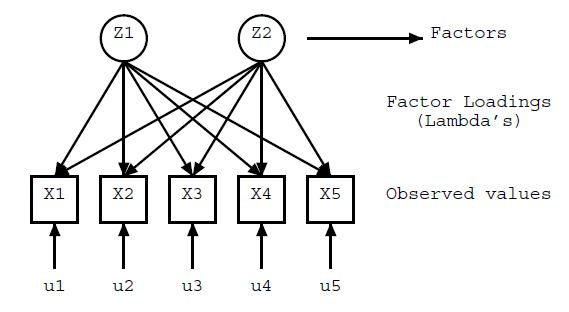
\includegraphics[width=0.6\columnwidth]{images_fractal/frac_1.JPG}
\caption{ Simple route diagram for a factor analysis model }
\label{fig:fig_1}
\end{figure}

The objective of the factor analysis is to find $\Lambda$ and $\Psi$ which improves the model of the $ x $ structure. The factorial variables $ z $ of the correlation model between the elements of $ x $, while the variable $ u $ counts for an independent noise in each element of $ x $. The $ m$ factors play the same role of principal components in the PCA. We first subtract the information from the data and then show the date as:
\begin{equation}
    x - \mu = \Lambda z + u
\end{equation}

\subsection{Self Supervised Multi Layer Perceptrons}
The supervised MLP architecture, or also called autoencoder, implements a mapping using two layers of linear perceptrons with $ d $ input, $ m $ hidden units and $ d $ training outputs to replicate the input to the output layer minimizing the error Of the sum of squares with \textit{backpropagation}. This approach is called \textit{self-supervised}, referring to the fact that during training each vector output sample is identical to the vector input sample.
\begin{figure}[htp]\centering
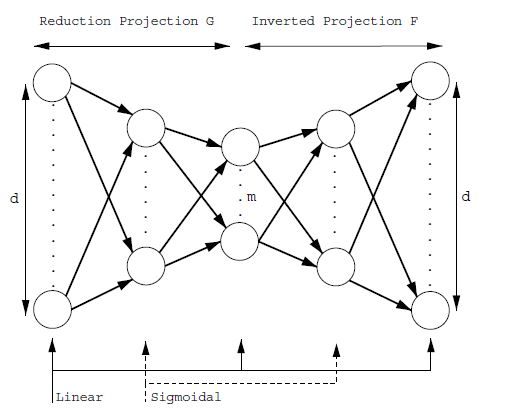
\includegraphics[width=0.6\columnwidth]{images_fractal/frac_2.JPG}
\caption{ The self-supervised MLP architecture }
\label{fig:fig_2}
\end{figure}

A botleneck MLP with a unique hidden layer physically performs a linear PCA even with non-linear hidden units. In fact, in order to effectively implement a non-linear dimensionality reduction, the mapping function $ F $ and $ G $ must be both non-linear. The process of dimensionality reduction consists to find the functions $ F $ and $ G $ which are approximately functions inverse to each other. Since the inverse of a nonlinear function can not be linear, therefore, if any of the functions is linear, the other must also be linear.

Linear self-supervised MLP can be extended to implement a non-linear PCA, using non-linear activation functions and more hidden layers (see Figure \ref{fig:fig_2}).

\section{SUPERVISED HASHING: A SIMPLE BASELINE}

%This section describes the protocols used in the literature for SSH and SH, and discuss how a simple strategy efficiently solves the corresponding problems.

In this section, we describe the protocols used in the literature for SSH and SH and explain how a simple strategy efficiently solves the similar problems.

\subsection{Evaluation protocols of SSH and SH}

%The task of SSH consists in indexing a dataset of $N$ images $\mathcal{I}_{train}$, of which a subset $\mathcal{I}_{label} \subseteq \mathcal{I}_{train}$ is labeled.  SH is the extreme case $\mathcal{I}_{label} = \mathcal{I}_{train}$. Given an unlabeled query image $q$, the system must return an ordered list of images from the $\mathcal{I}_{train}$. For evaluation purposes, a dataset of queries is given; the labels of the queries as well as all labels in $\mathcal{I}_{train}$ are known to the evaluator, even in the SSH setting, and an image is deemed correct if it has the same label as the query. The performance is measured in terms of precision or mean average precision (mAP), which we now describe.
SSH consists in index a dataset of $N$ images $\mathcal{I}_{train}$, of which a subset $\mathcal{I}_{label} \subseteq \mathcal{I}_{train}$ is labeled.  But, SH is the extreme case $\mathcal{I}_{label} = \mathcal{I}_{train}$. If we have an unlabeled query image $q$, the system have to return an ordered list of images from the $\mathcal{I}_{train}$. To evaluate, we have a dataset of queries; the evaluator knows all labels of the queries as well as the labels in $\mathcal{I}_{train}$, also in the SSH setting, then an image is considered correct if it and query have the same label. The performance is measured by precision or mean average precision (mAP).

%Given a query $q$, we first define $\delta (q, i)=1$ if the $i^{th}$ image is correct for $q$, and $0$ otherwise. The precision at (rank) $k$ is given by $P(q,k) = \tfrac{1}{k} {\sum}_{i=1}^{k} \delta (q, i)$. Denoting by $cl(q) = {\sum}_{i=1}^{N} \delta (q, i)$ the total number of correct images in $\mathcal{I}_{train}$, the average precision at $k$ is $AP(q, k) = \tfrac{1}{cl(q)}{\sum}_{i=1}^{k}\delta (q, i) P(q,i)$. The mAP at $k$ (or simply mAP when $k = N$) is the mean AP over all test queries.
Then, given a query $q$, if the $i^{th}$ image is correct for $q$ we define $\delta (q, i)=1$ , and $0$ otherwise. The precision at (rank) $k$ is given by $P(q,k) = \tfrac{1}{k} {\sum}_{i=1}^{k} \delta (q, i)$. Denoting by $cl(q) = {\sum}_{i=1}^{N} \delta (q, i)$ the total number of correct images in $\mathcal{I}_{train}$, and the average precision at $k$ is $AP(q, k) = \tfrac{1}{cl(q)}{\sum}_{i=1}^{k}\delta (q, i) P(q,i)$. The mAP at $k$ (or simply mAP when $k = N$) is the mean AP over all test queries.

\subsection{Retrieval through class probability estimation}

%The information retrieval \cite{doi:10.1108/eb026647} and learning to rank that the optimal prediction for precision at $k$ is given by ranking items $x \in \mathcal{I}_{train}$ n according to their probability of being correct for the query. This result extends to the optimization of $mAP$.

The information recovery \cite{doi:10.1108/eb026647} and learning to rank that the best prediction for precision at $k$ is given by placing items $x \in \mathcal{I}_{train}$ n according to their probability of being correct for the query. This result extends to the optimization of $mAP$.
\\
%\textbf{Optimal ranking for SH.} In the specific setup of SH where the system knows the labels of the images in $\mathcal{I}_{train}$, the probability that an image $x$ with label $y$ is correct is the probability $\mathbb{P}(y\mid q)$ that the query image has label $y$. The important point here is that the probability of $x$ being correct for $q$ only depends on the label of $x$. Thus, ordering the $C$ labels so that $\mathbb{P}(y\mid q)\geq \dots \geq\mathbb{P}(c_C\mid q)$,the optimal ranking is to return all images of $\mathcal{I}_{train}n$ with label $c_1$ first, followed by all images with label $c_2$, and so on.
\textbf{Optimal ranking for SH.} In the particular setup of SH where the system knows the labels of the images in $\mathcal{I}_{train}$, the probability that a picture $x$ with label $y$ is correct is the likelihood $\mathbb{P}(y\mid q)$ that the query image has label $y$. The important point in this part is that the probability of $x$ being correct for $q$ only depends on the label of $x$. Thus, ordering the $C$ labels so that $\mathbb{P}(y\mid q)\geq \dots \geq\mathbb{P}(c_C\mid q)$, the best ranking is to return the complete dataset of $\mathcal{I}_{train}n$ with label $c_1$ first, followed by all the pictures with label $c_2$, and so on.
\\
\begin{comment}
In practice, $\mathbb{P}(.\mid q)$ is unknown, but we can train a classifier
on $\mathcal{I}_{label} = \mathcal{I}_{train}$ which outputs probability estimates $\hat{\mathbb{P}}(c\mid q)$ for every label $c$, and compute the optimal ranking according to $\hat{\mathbb{P}}(c\mid q)$ Such probability estimates are given by,
e.g., multiclass logistic regression or a Convolutional Neural
Network (CNN) with a softmax output layer. Labels of $ \mathcal{I}_{train}$
are stored on [$log2 (C)$] e bits or in an inverted file.
\end{comment}

In practice, $\mathbb{P}(.\mid q)$ is unfamiliar, but we can train a classifier on $\mathcal{I}_{label} = \mathcal{I}_{train}$ which outputs probability con predict $\hat{\mathbb{P}}(c\mid q)$ for every label $c$, and process the optimal ranking according to $\hat{\mathbb{P}}(c\mid q)$ Such probability estimates are shown by, e.g., multiclass logistic regression or a Convolutional Neural
Network (CNN) with a softmax output layer. Labels of $ \mathcal{I}_{train}$
are stored on [$log2 (C)$] e bits or in an inverted file

\\\\
%\textbf{Relationship between classification accuracy and ranking performance.} If we denote the classification accuracy as $p$, then the resulting mAP is at least $p$. When the classifier predicts the class of $q$ correctly, all images of that class will be ranked first and the resulting AP($q$) is $1$; this happens on a proportion $p$ of the queries. So, the classification accuracy is a lower bound on the mAP.

\textbf{Relationship between classification accuracy and ranking performance.} If we show the classification accuracy as $p$, then the resulting $mAP$ is at least $p$. When the classifier foretells the class of $q$ properly, all images of that class will be ranked first, and the resulting AP($q$) is $1$; this happens on a proportion $p$ of the queries. So, the classification accuracy is a lower bound on the mAP.
\\\\
%\textbf{Optimal ranking for SSH.} In the more general setup of SSH, we do not know the label of some images in $\mathcal{I}_{train}$. Yet, considering the (true) conditional label probabilities $\mathbb{P}(c\mid q)$ and $\mathbb{P}(c\mid x)$, the probability that $x$ is correct for $q$ is given by $\sum_{c=1}^C \mathbb{P}(c\mid q) \mathbb{P}(c\mid x) $ it is the probability that both q and x have the same label, assuming conditional independence of the labels of the query and the image. Notice that this is the dot product between the conditional label probability vectors of $q$ and $x$.Then, given probability estimates $\hat{\mathbb{P}}$  for the labels of queries and images, which are obtained on $\mathcal{I}_{label}$, we consider two retrieval algorithms:
\textbf{Optimal ranking for SSH.} In the more general setup of SSH, we do not know the label of some images in $\mathcal{I}_{train}$. Yet, considering the (real) probabilities $\mathbb{P}(c\mid q)$ and $\mathbb{P}(c\mid x)$, the probability that $x$ is correct for $q$ is given by $\sum_{c=1}^C \mathbb{P}(c\mid q) \mathbb{P}(c\mid x) $ it is the probability that both q and $x$ have the same label, assuming conditional self-sufficiency of the labels of the query and the image. Notice that this is the dot product between the dependent label probability vectors of $q$ and x$. Then, given probability measures $\hat{\mathbb{P}}$  for the labels of queries and images, which are taken on $\mathcal{I}_{label}$, we consider two retrieval algorithms:

\\\\
\begin{itemize}
%\item \textbf{Classifier topline: }: For each image $x$of $\mathcal{I}_{train}$, store a vector $u(x)$ equal to either (1) the one-hot encoding vector of the label of $x$ if $x \in \mathcal{I}_{label}$, or (2) the full conditional probability vector  $\hat{\mathbb{P}}(.\mid x)$). Rank images $x$ according to the dot product $\langle\hat{\mathbb{P}}(.\mid q), u(x)\rangle$  This strategy corresponds to the optimal strategy, but requires storing the probability vectors for images in $\mathcal{I}_{train} \backslash \mathcal{I}_{label}$

\item \textbf{Classifier topline: }: For each image $x$of $\mathcal{I}_{train}$, saves a vector $u(x)$ equal to either (1) the one-hot encoding vector of the label of $x$ if $x \in \mathcal{I}_{label}$, or (2) the full  vector  $\hat{\mathbb{P}}(.\mid x)$). Rank images $x$ according to the dot product $\langle\hat{\mathbb{P}}(.\mid q), u(x)\rangle$  This strategy corresponds to the best strategy, but needs to save the probability vectors for each image in $\mathcal{I}_{train} \backslash \mathcal{I}_{label}$

%\item \textbf{Classifier hashed: } Here we hash the conditional probability vector. The first hashing method that we evaluate, is the one-hot strategy, which stores the index of the maximal activation on $\left \lceil log_2(C) \right \rceil$ bits. This approach, denoted \textbf{Classifier+one-hot} in what follows, returns all images of the strongest class first. The second encoding, referred to as Classifier+LSH, is locality-sensitive hashing (LSH) with tight frames \cite{jegou2012anti}, a simple non data adaptive hashing scheme. This LSH method produces binary vectors that are compared with Hamming distances. Therefore it can be used as drop-in replacements for the competing binary encoding methods.

\item \textbf{Classifier hashed: } Here we hash the probability vector. The first hashing method that we evaluate, is the one-hot strategy, which saves the index of the maximal activation on $\left \lceil log_2(C) \right \rceil$ bits. This approach, expressed \textbf{Classifier+one-hot} in what results, returns all images of the strongest class first. The second encoding, referred to as Classifier+LSH, is locality-sensitive hashing (LSH) with tight frames \cite{jegou2012anti}, a simple non data adaptive hashing scheme. This LSH method provides binary vectors that are compared with Hamming distances. Consequently it can be used as drop-in replacements for the competing binary encoding methods.
\end{itemize}

















\section{How should we evaluate supervised hashing?}

\subsection{HASHING FOR NEAREST NEIGHBOR SEARCH}
Compress a set of vectors $(x_i)^{b}_{i=1}, x_i \in \mathbb{R}^{d}$
\begin{figure}[htp]
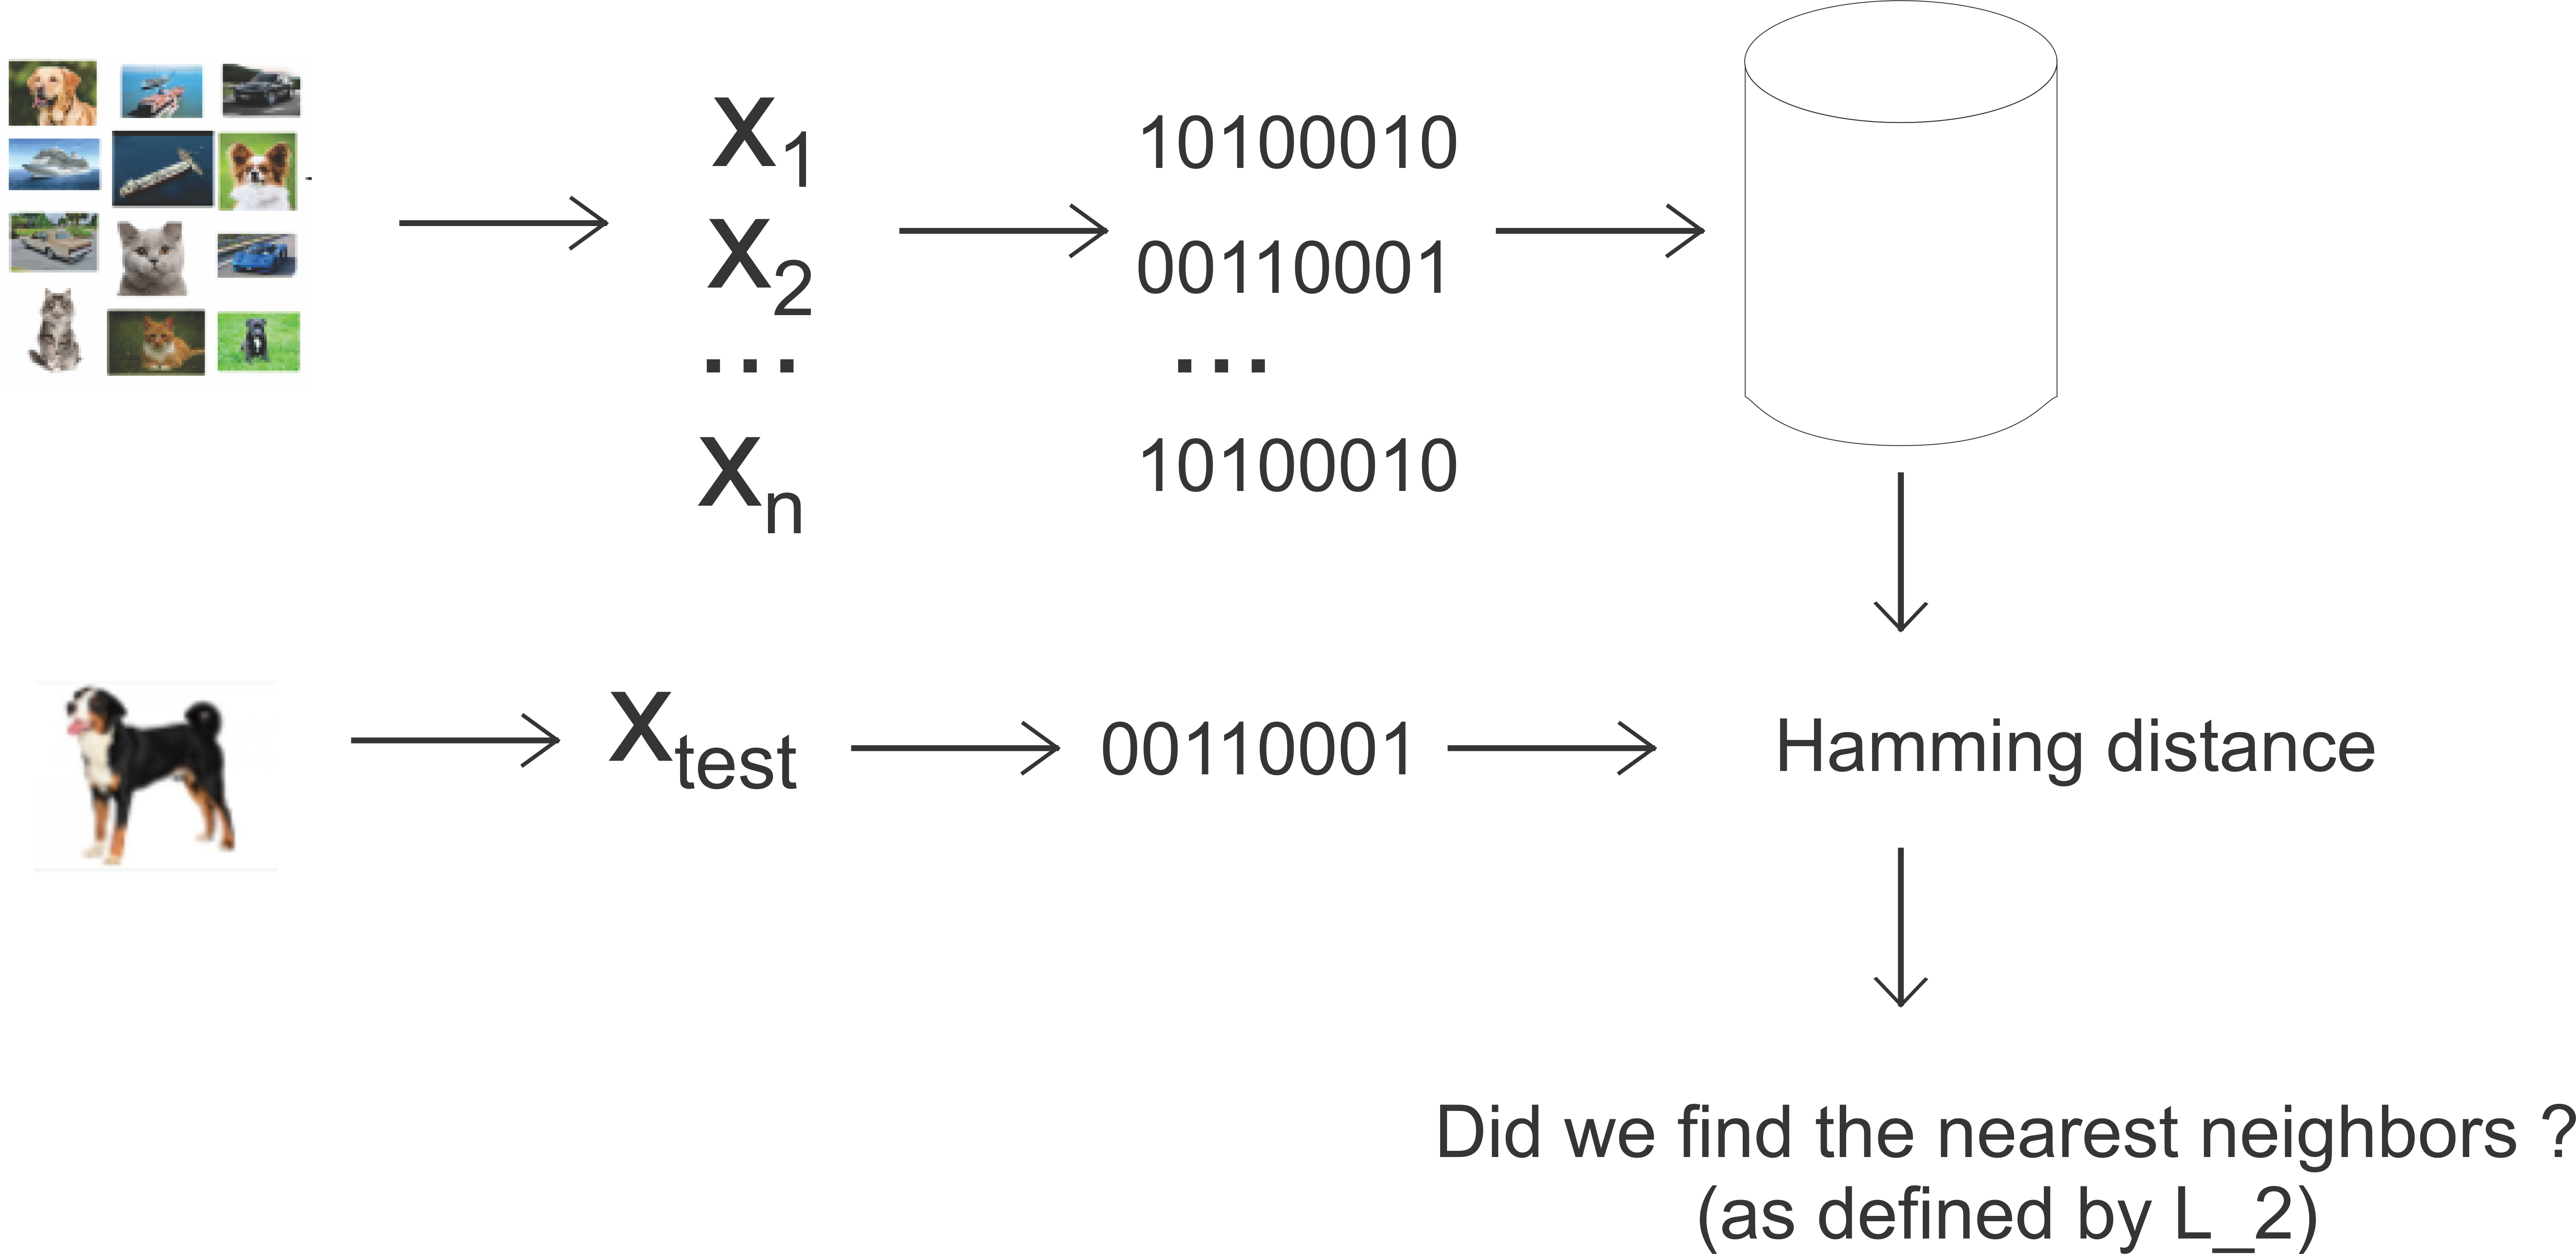
\includegraphics[width=8cm]{dash/11.PNG}
\centering
\end{figure}

\subsection{SUPERVISED HASHING}
Compress a set of vectors and their labels  $((x_i,y_2))^{n}_{i=1}, x_1\in \mathbb{R}^{d}, y_1 \in \{1,...,L\} $
\begin{figure}[htp]
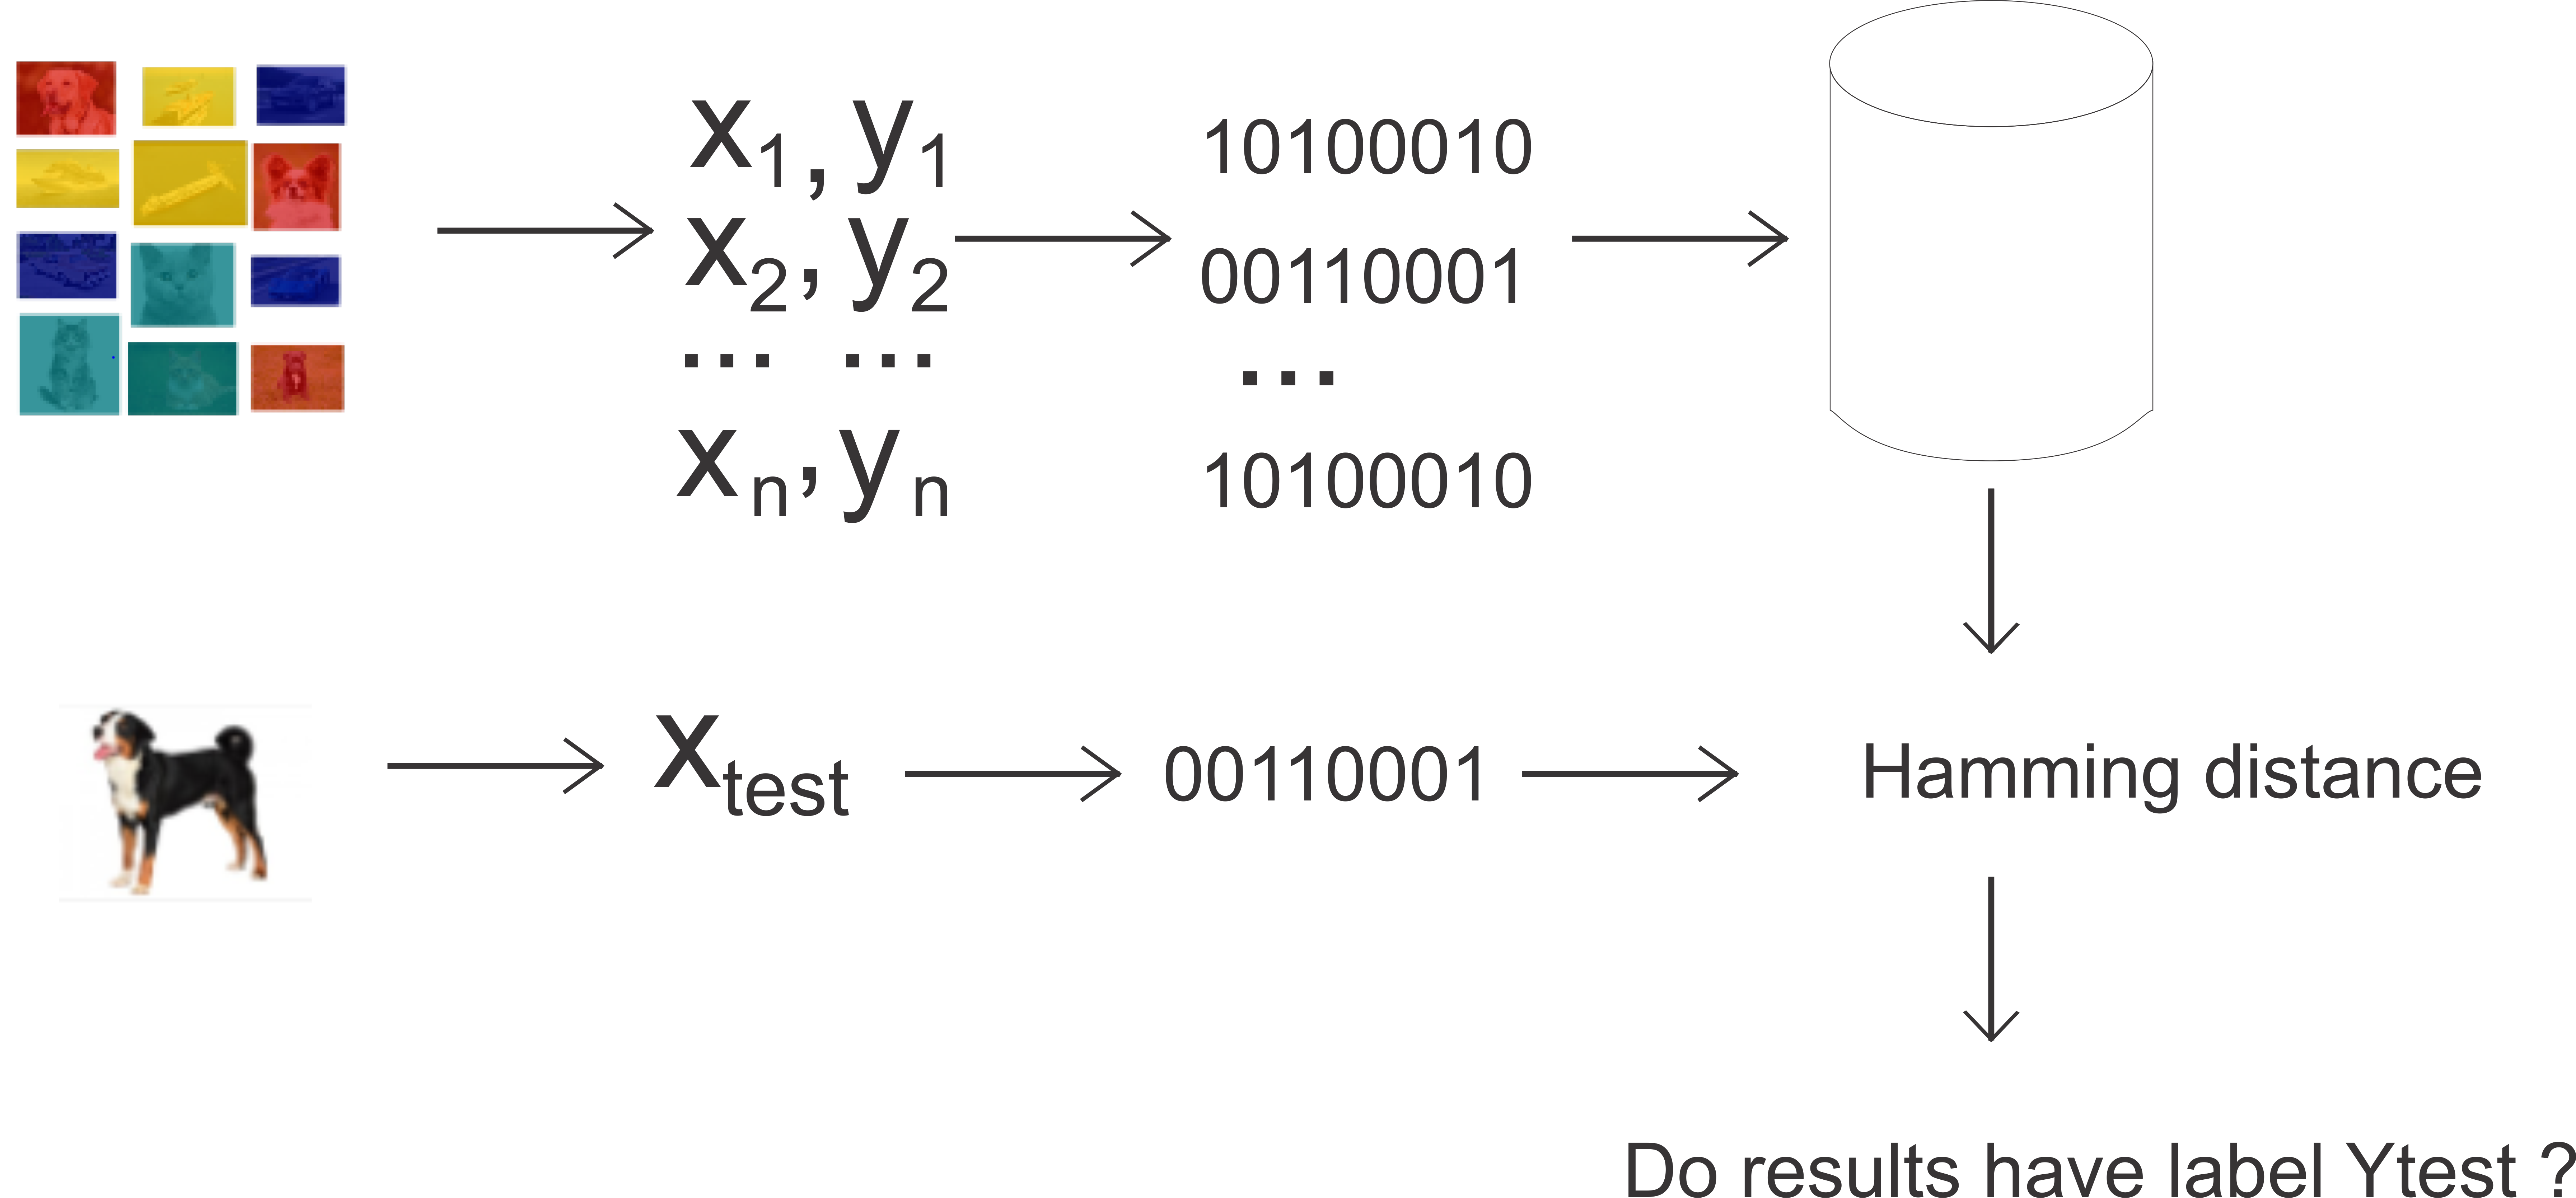
\includegraphics[width=8cm]{dash/12.png}
\centering
\caption{ HASHING FOR NEAREST NEIGHBOR SEARCH }
\end{figure}

\begin{itemize}
\item Supervised hashing $[1, 2]$: labels $y$ known for all $x$ in the reference set
\item Semi-supervised hashing $[3, 4]$: labels $y$ known for only $n_label$ samples
\end{itemize}

\subsection{WHY NOT JUST ENCODE THE CLASS ID?}
Supervised hashing with classification baseline
\begin{itemize}
\item Trivial binary encoding of the class id,$ e.g. y=9 \rightarrow 1001$
\centering

\begin{eqnarray}
\cancel{x_1}, y_1  & & 1001    \\
\cancel{x_2}, y_2  & \rightarrow & 1001   \\
\dots  & & \dots \\
\cancel{x_n}, y_n  & & 0011
\end{eqnarray}
\item Train classifier on pairs $(x_1, y_1),  \dots ,(x_n; y_n)$ and predict $y_test$ with the classifier
\item Guaranteed performance: $mAP \geq$ classifier accuracy
\end{itemize}

\subsection{EXTENSION TO SEMI-SUPERVISED HASHING}
\begin{equation}
\begin{split}
    \mathbb{P}(x\;correct for\; q) & = \sum_{j=label} \mathbb{P}(j\mid x)\mathbb{P}(j\mid q)  \\
    &=(\mathbb{P}(j\mid x),\mathbb{P}(j\mid q))  \\
    &=\underbrace{(\hat{\mathbb{P}}(j\mid x)}_{classifier},\hat{\mathbb{P}}(j\mid q))  \\
\end{split}
\end{equation}
\begin{itemize}
    \item Train $\hat{\mathbb{P}}$ on labelled images
    \item Compute $\hat{\mathbb{P}}(\cdot\mid x) \in\left[0,1\right]^{L}$ for $x$ unlabelled
    \item Compress $\hat{\mathbb{P}}(\cdot\mid x)$ with one-hot / LSH
\end{itemize}

\begin{table}[]
\centering
\caption{Results on CIFAR-10}
\label{my-label}
\begin{tabular}{|l|l|l|l|l|l|}
\hline
Features & $n_label$ & $n_anchors$ & Method                                                                                    & bits                                                         & mAP                                                                           \\ \hline
GIST     & 59,000    & 1,000       & \begin{tabular}[c]{@{}l@{}}SQ{[}1{]}\\ SQ{[}1{]}\\ One-hot\end{tabular}                   & \begin{tabular}[c]{@{}l@{}}64\\ 128\\ 4\end{tabular}         & \begin{tabular}[c]{@{}l@{}}0.704\\ 0.712\\ 0.762\end{tabular}                 \\ \hline
GIST     & 5,000     & 1,000       & \begin{tabular}[c]{@{}l@{}}SDH{[}3{]}\\ One-hot\\ LSH\\ Topline\end{tabular}              & \begin{tabular}[c]{@{}l@{}}64\\ 4\\ 64\\ -\end{tabular}      & \begin{tabular}[c]{@{}l@{}}0.402\\ 0.377\\ 0.430\\ 0.578\end{tabular}         \\ \hline
GIST     & 1,000     & 300         & \begin{tabular}[c]{@{}l@{}}KSH{[}4{]}\\ KSH{[}4{]}\\ One-hot\\ LSH\\ Topline\end{tabular} & \begin{tabular}[c]{@{}l@{}}12\\ 48\\ 4\\ 48\\ -\end{tabular} & \begin{tabular}[c]{@{}l@{}}0.232\\ 0.284\\ 0.270\\ 0.309\\ 0.350\end{tabular} \\ \hline
DEEP     & 50,000    & -           & \vdots                                                                                    & \vdots                                                       & \vdots                                                                        \\ \hline
AlexNet  &           &             & \begin{tabular}[c]{@{}l@{}}DSH{[}2{]}\\ DSH{[}2{]}\\ One-hot\end{tabular}                 & \begin{tabular}[c]{@{}l@{}}12\\ 48\\ 4\end{tabular}          & \begin{tabular}[c]{@{}l@{}}0.616\\ 0.621\\ 0.870\end{tabular}                 \\ \hline
\end{tabular}
\end{table}
\begin{table}[]
\centering
\caption{Results on ImageNet}
\label{my-label}
\begin{tabular}{llll}
Features & Method    & bits & mAP@1500 \\
VGG      & SQ{[}1{]} & 128  & 0.620    \\
VGG      & one-hot   & 10   & 0.664
\end{tabular}
\end{table}

\textbf{Encoding schemes}
\begin{itemize}
\item One-hot:$(0.15,0.07,0.08,\textbf{0.7})\rigtharrow 3 \rigtharrow 0011$
\item LSH:$(0.15,0.07,0.08,0.7)\rigtharrow (sign(w_i^T \cdot v + b_i))_{i=1}^{n_bits}$
\item Top line: no compression
\end{itemize}

\subsection{HOW CAN WE AVOID THIS BIASED PROTOCOL?}
\ref{fig:13}.
\begin{figure*}[htp]\centering
\label{fig:13}
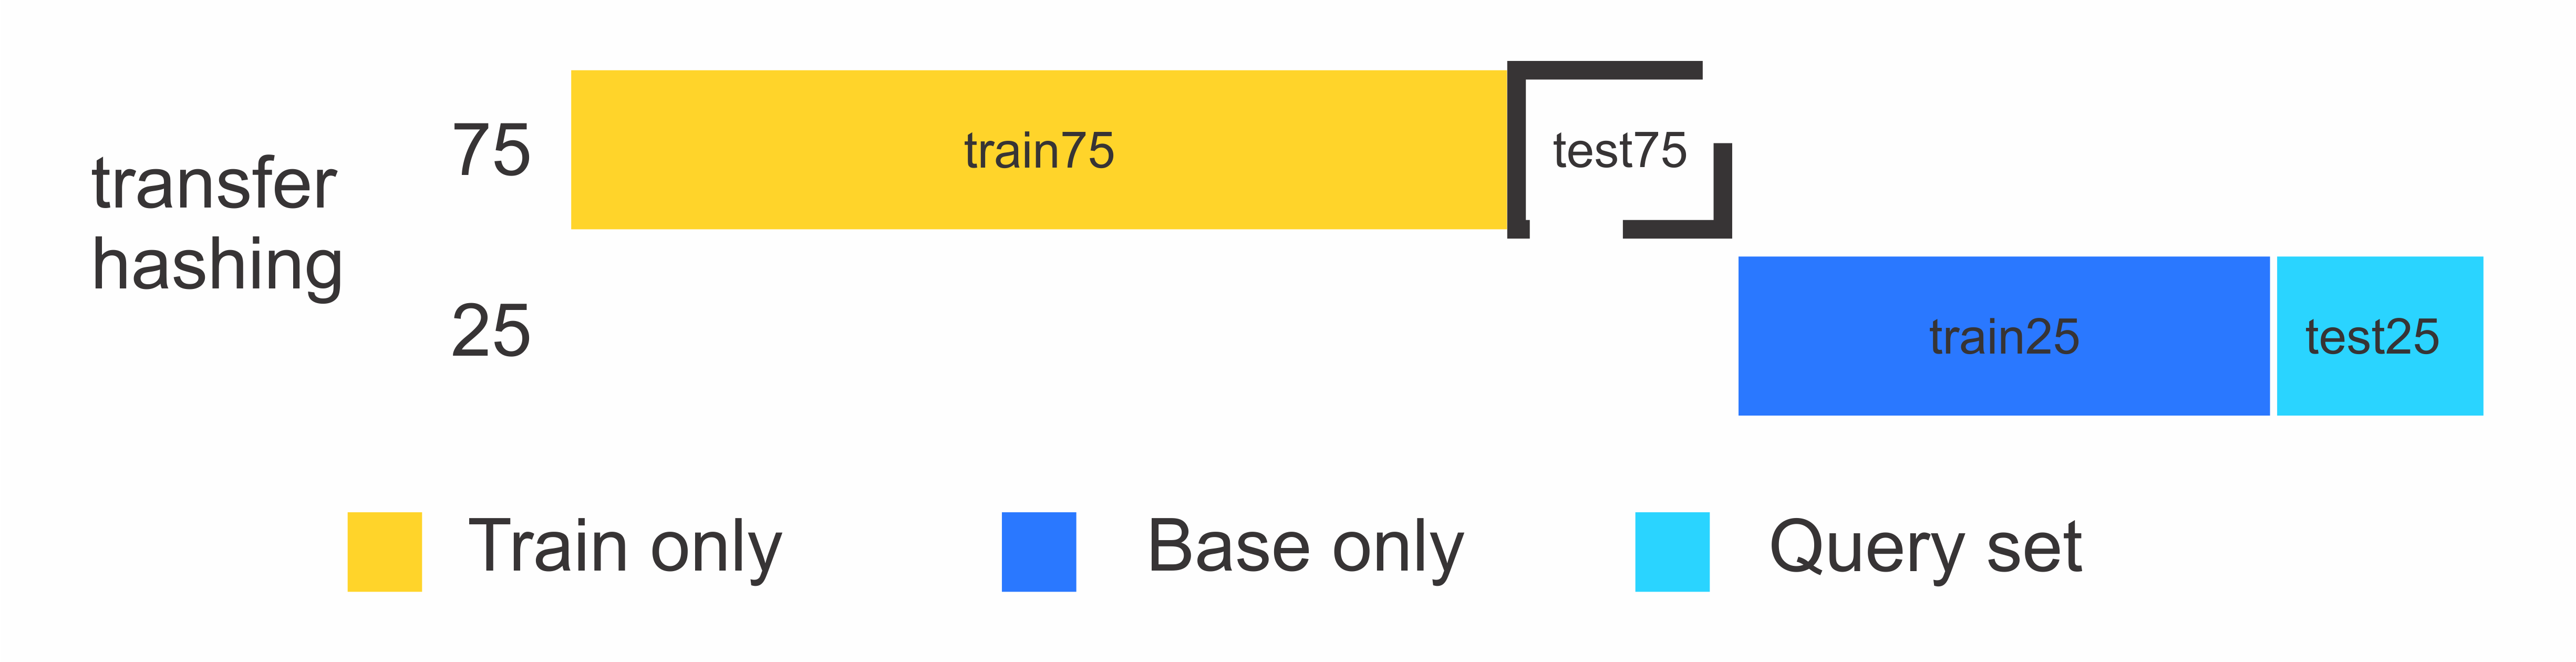
\includegraphics[width=8cm]{dash/13.png}
\end{figure*}

\begin{itemize}
\item Test on classes \textbf{never seen at train time}
\itemSplit classes in 4 folds, each with 25\% of classes,Both setups:
    \begin{itemize}
    \item Train hash functions on train75
    \item Encode train25 with hash functions
    \end{itemize}
\item \textbf{Setup 1: Retrieval with hash codes}
    \begin{itemize}
    \item Use train25 as reference set
    \item Use test25 as queries
    \end{itemize}
\item \textbf{Setup 2: Classification on hash codes}
    \begin{itemize}
    \item Train classifier using train25 labels
    \item Evaluate accuracy on test25
    \end{itemize}
\end{itemize}

\subsection{UNSUPERVISED BASELINE FOR PROPOSED PROTOCOL}
\begin{itemize}
\item \textbf{Experimental setting}
    \begin{itemize}
    \item Experiments with CIFAR-10 using AlexNet
    \item Unsupervised PQ codes [5] with 4 bytes
    \end{itemize}
\item \textbf{Setup 1: Retrieval with hash codes}
    \begin{itemize}
    \item PQ codes with asymmetric comparison
    \item Higher layers are better
    \item 4 bytes enough for most of performance
    \item Inner product on softmax gets the best result
    \end{itemize}
\item \textbf{Setup 2: Classification on hash codes}
    \begin{itemize}
    \item Drop in accuracy due to encoding
    \item Lower layers more generic$\rightarrow$better accuracy
    \item Lower layers high dimensional$\rightarrow$larger gap between PQ and full vector
    \item $\rightarrow$ Trade-off encoding/accuracy
    \end{itemize}
\end{itemize}
 








\section{EVALUATION PROTOCOLS}

In this section, we describe the two evaluation tasks proposed in \cite{sablayrolles2016should}, namely retrieval of unseen classes, and transfer learning to new classes. They correspond to application cases on large datasets. The two protocols differ only in the evaluation metric: ranking versus class accuracy.

\textbf{Dataset definition.} at test time we use separate classes from a standard classification dataset. When learning the hashing function $75\%$ of the classes are assumed to be known, and the $25\%$ remaining classes are used to evaluate the encoding/hashing scheme. We call train75/test75 the train/test images of the $75\%$ classes and train25/test25 the remaining ones.

\textbf{Protocol 1: Retrieval of unseen classes}, to index train25 and use test25 as queries, we use the hashing scheme. We use the labels of train25 for evaluation only. This setup is like an instance search approach except that the class labels give the ground-truth. The train75 - train25 - test25 split is the supervised equivalent of the learn - database - query split in unsupervised hashing.

\textbf{Protocol 2: Transfer learning, } the authors proposed to train a new CNN from scratch with the same structure as the top of the original network, using the stored train25 descriptors. The goal is to maximize the transfer accuracy on test25.

\section{Experiments}

In this section, we are interested in answering the following question: (a) How accurate is our model in estimating the LSH parameters using the fractal dimension; (b) How does our DAsH method  improve the other LSH implementations in terms of \textit{querying performance} and \textit{precision}. The performance of DAsH method was compared to  two   well-known approximate search methods, namely  Multi-probe LSH \cite{multiprobe}, LSH-Forest \cite{lshforest}, ITQ \cite{itq}, and LOPQ \cite{lopq}. All of the experiments were performed on a workstation with Intel core i7  3.0Ghz (12 cores) CPU and 64Gb RAM which is supplied with four Geforce GTX 1080 GPU with 8Gb VRAM each one.

We first conduct experiments on eight  widely used datasets using hand-crafted features (AUDIO, CITIES, EIGENFACES, HISTOGRAMS, MGCOUNTY, RANDOMWALK, SYNTH16D, SYNTH6D, VIDEO)\footnote{\url{https://github.com/joselhuillca/fractal_dataset}} to evaluate our proposed  method for   estimating the LSH parameters. Beside hand-crafted features, we also show the effectiveness of our methods when deep features   are extracted by the deep Convolutional Neural Networks (CNN),  we conduct this experiment on three datasets (MNIST\footnote{\url{http://yann.lecun.com/exdb/mnist/}}, CIFAR-10\footnote{\url{https://www.cs.toronto.edu/~kriz/cifar.html}}, SVHN\footnote{\url{http://ufldl.stanford.edu/housenumbers/}}) to evaluate our in terms of querying performance,  meap average precision (mAP), and precision. The following describes the details of the experiments and results.

 





\subsection{Experiment 1: Tunning LSH Parameters}

LSH based methods report efficient results when adequate values for $m$ (number of hash functions) are chosen. To evaluate the effectiveness of the presented approach to tune the LSH parameters using fractal dimension, we worked on a variety of synthetic and real dataset. Table \ref{table:lshparams} summarizes the main features and parameters of the datasets, including the number of elements $N$, number of attributes $d$,   their intrinsic (fractal) dimension $\mathfrak{D}$, the LSH parameters computed using two approaches: the Andoni \footnote{\url{http://www.mit.edu/~andoni/LSH/}} algorithm and our proposal based on fractal dimension, and the total computation time for tune the LSH index (in seconds).  The experiment results for the number of hash functions $m$  show that the estimations given by Equation \ref{eq:fractalm} are comparable with those obtained with the E2LSH algorithm proposed by Andoni using up to $10X$ less time.
 


\subsection{Retrieval Performance} % OK
 The aim of this experiment is to measure the total time   spent  retrieving the $k$-nearest neighbor objects. The data structures being compared were tested with an specific values for queries. Thus we use   $k=1000$   when compute the Mean Average Precision($mAP$) metric and $k=25$ when compute the  precision metric $(P (\%))$.
 

\begin{table*}[ht]
\centering
\caption{My caption}
\label{my-label}
\begin{tabular}{|l|r|r|r|r|r|r|r|}
\hline
                     & \multicolumn{6}{c|}{\textbf{SMALL SPACE}}                 & \multicolumn{1}{l|}{\textbf{ORIG. SPACE}} \\ \hline
\multicolumn{8}{|c|}{\textbf{AGNEW}}                                                                                         \\ \hline
\textbf{Dim}         & 16      & 32      & 64      & 128     & 256     & 512     & 8704                                      \\ \hline
\textbf{Fractal Dim} & 4.2656  & 4.5797  & 5.7044  & 20.5952 & 24.7651 & 24.7651 & 30.4943                                   \\ \hline
\multicolumn{8}{|c|}{\textbf{CIFAR10}}                                                                                       \\ \hline
\textbf{Dim}         & 16      & 32      & 64      & 128     & 256     & 512     & 4096                                      \\ \hline
\textbf{Fractal Dim} & 1.4436  & 5.4327  & 7.2287  & 23.2534 & 25.5753 & 25.5753 & 1.6494                                    \\ \hline
\multicolumn{8}{|c|}{\textbf{ISBI}}                                                                                          \\ \hline
\textbf{Dim}         & 16      & 32      & 64      &         &         &         & 4096                                      \\ \hline
\textbf{Fractal Dim} & 11.6047 & 16.1283 & 16.1283 &         &         &         & 16.1283                                   \\ \hline
\multicolumn{8}{|c|}{\textbf{MNIST}}                                                                                         \\ \hline
\textbf{Dim}         & 16      & 32      & 64      & 128     & 256     &         & 800                                       \\ \hline
\textbf{Fractal Dim} & 4.3912  & 4.1542  & 22.5753 & 22.5753 & 22.5753 &         & 22.5753                                   \\ \hline
\multicolumn{8}{|c|}{\textbf{SVHN}}                                                                                          \\ \hline
\textbf{Dim}         & 16      & 32      & 64      & 128     &         &         & 1152                                      \\ \hline
\textbf{Fractal Dim} & 6.5841  & 4.6553  & 28.3359 & 28.3359 &         &         & 28.3359                                   \\ \hline
\end{tabular}
\end{table*}

\section{Conclusions}
 


\bibliographystyle{plain}
\bibliography{references}

\end{document}

